\section{Introduction}
\label{sec:intro}

Start with the problem and why it matters. Symmetry is one of the most reliable inductive biases in machine learning for the physical sciences: a model whose outputs transform predictably under rotations, translations or permutations needs less data and generalizes further~\cite{bronstein2021geometric,cohen2016group}. \Cref{fig:teaser} shows how a figure, its caption and a cross-reference look in this template.

\begin{figure}[t]
  \centering
  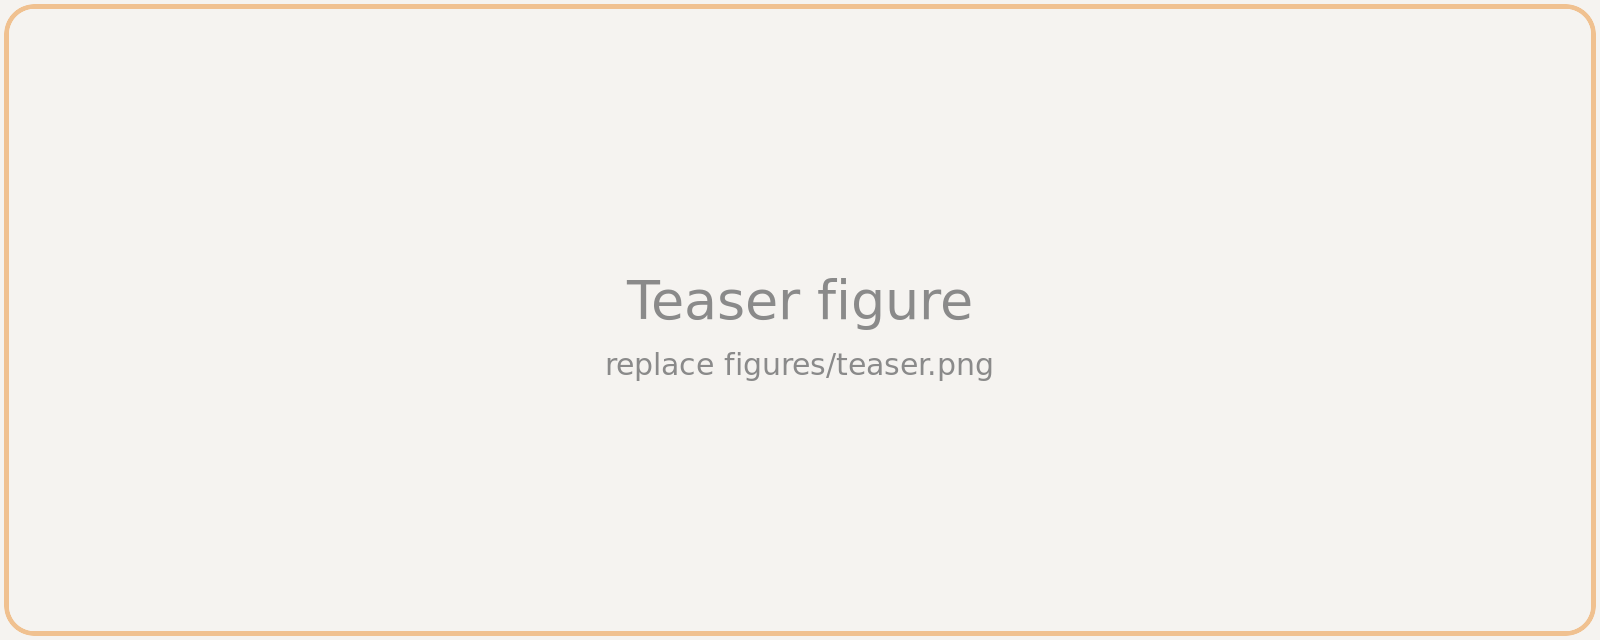
\includegraphics[width=0.82\linewidth]{figures/teaser}
  \caption{\textbf{Teaser figure.} Replace this placeholder with the figure that best summarizes the paper. Captions open with a bold one-line takeaway, then explain what the reader should look at.}
  \label{fig:teaser}
\end{figure}

\parahead{Contributions} State them as a short list.
\begin{itemize}
  \item A new model, \method, that is equivariant by construction (\cref{sec:method}).
  \item A theoretical guarantee on its expressivity (\cref{thm:main}).
  \item Experiments on simulated and real robotic systems (\cref{sec:experiments}).
\end{itemize}

\subsection{Related work}
Group related work by theme in short paragraphs, cite with \verb|\cite|~\cite{vaswani2017attention}, and close with one sentence on how the present work differs.
